\chapter{Multi-Armed Bandits \cite{medium-numsmt2-rl-ch2-part-1,umich-teneket-MAB,arxiv-1904.07272}}\label{Multi-Arm Bandits}

\begin{table}[H]
    \centering
    \begin{minipage}{0.45\linewidth}
        \begin{figure}[H]
            \centering
            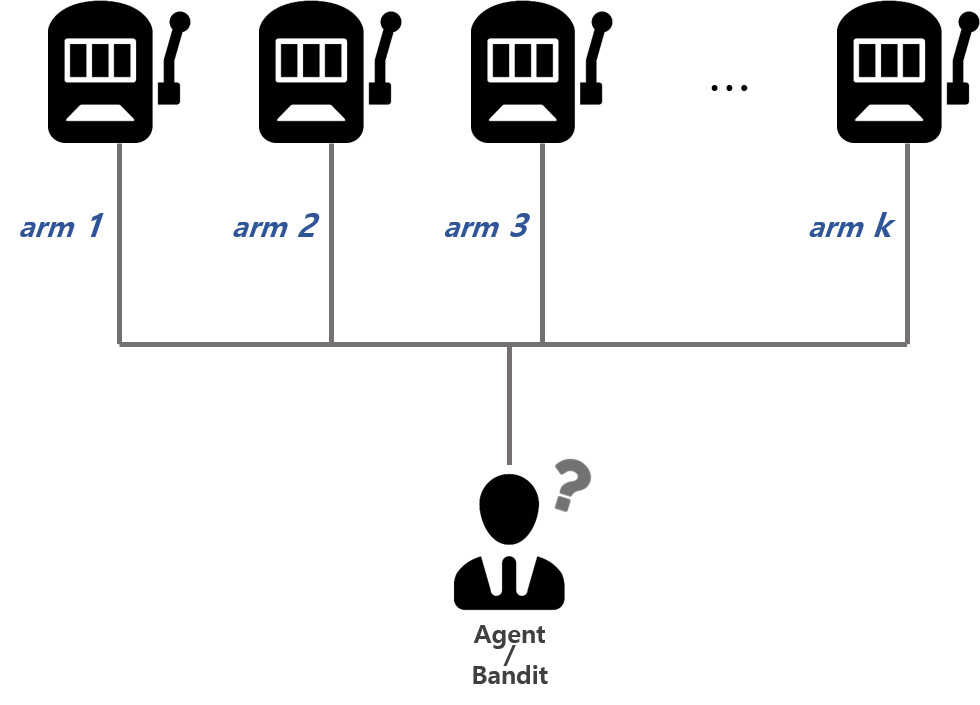
\includegraphics[height=5cm]{Pictures/deep-reinforcement-learning/multi-arm-bandit-1.jpg}
            \caption{Multi-Arm Bandit: Basic idea}
        \end{figure}
    \end{minipage}
    \hfill
    \begin{minipage}{0.45\linewidth}
        \begin{figure}[H]
            \centering
            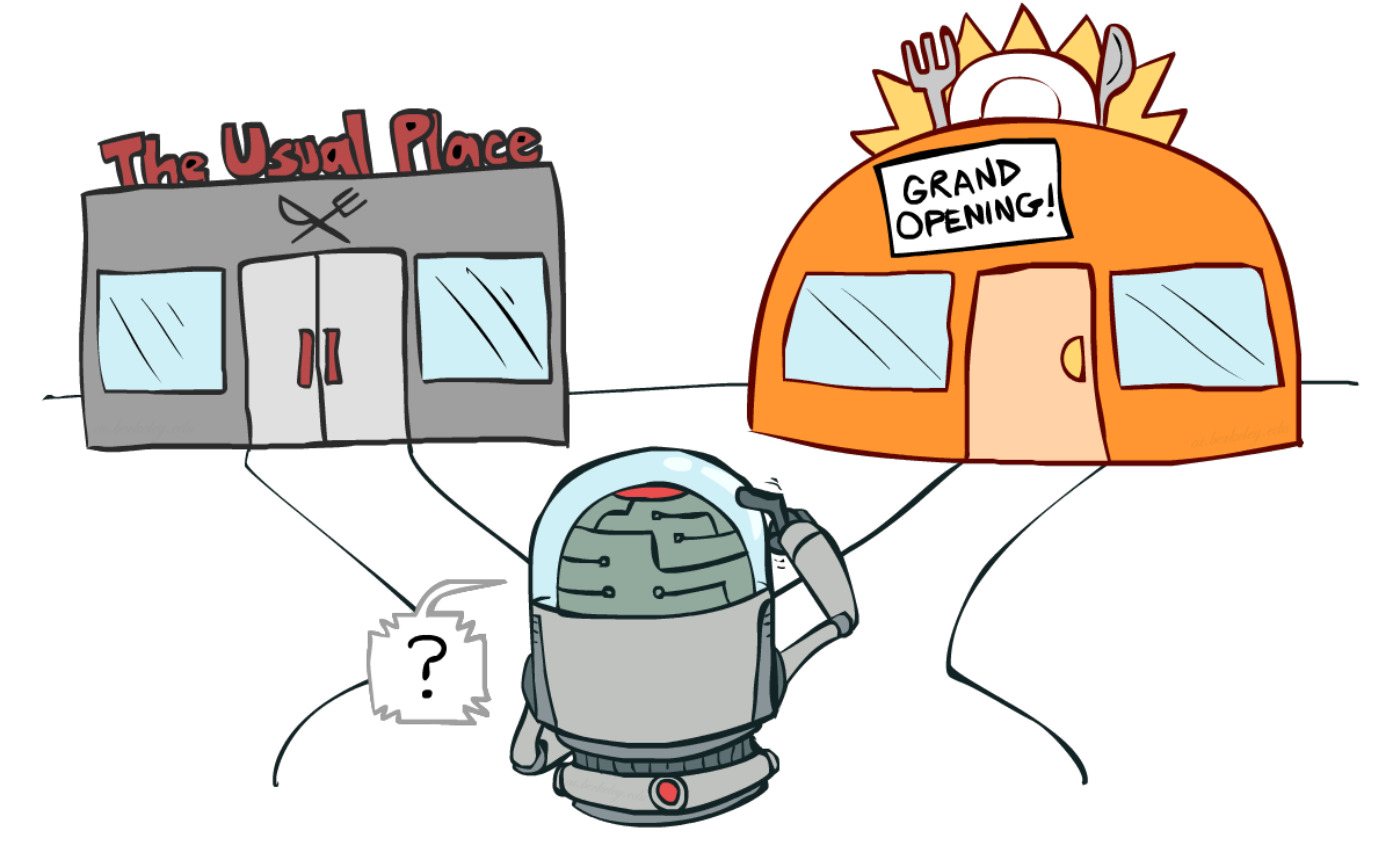
\includegraphics[height=5cm]{Pictures/deep-reinforcement-learning/multi-arm-bandit-2.jpg}
            \caption{Multi-Arm Bandit: Exploration vs Exploitation}
        \end{figure}
    \end{minipage}
\end{table}

\section{Intro to Multi-armed bandit}
Scenario: 
\begin{enumerate}
    \item we are in a casino, where we can choose any of the slot machines amongst the machines available.
    \item the winning probability of the machines is unknown to the user/ agent
\end{enumerate}
Multi-armed bandits is a simple but very powerful framework for algorithms that make decisions over time under uncertainty.\\
It is called Multi-armed bandits because slot machines (aka "One-armed Bandits") (as in casinos) were called bandits in earlier times because they loot people (winning probability is very less, so they keep loosing money).

\section{Notation \& Terminologies \cite{medium-numsmt2-rl-ch2-part-1}}
\begin{enumerate}
    \item $A_t$ : action taken at time t
    \item $R_t$ : reward at time t
    \item $q_*(a)$ : the value of any action $a$, defined as the expected reward for that action if it’s chosen \[
        q_*(a) = \mathbb{E}[R_t | A_t = a]
    \]\\[-0.5cm]
    i.e., the expectation ($E$) of getting some reward at time $t$ ($=R_t$) given that the action at time $t$ is $A_t = a$
    \item $Q_t(a)$ : estimated value of action $a$ at time $t$, (since we don’t know the actual value of any action we have to estimate)
\end{enumerate}

\vspace{0.2cm}
\noindent\textbf{Goal}: The goal is to get $Q_t(a)$ to be as close to $q_*(a)$ as possible. If we can closely estimate the true values of each action, we can know which actions to take to maximize reward.

\section{Exploration vs. Exploitation \cite{medium-numsmt2-rl-ch2-part-1}}\label{Exploration vs. Exploitation}
At any point in time there will be one action whose estimated value is highest, we call this action the \textbf{greedy action}\indexlabel{MAB: greedy action}.

\textbf{Exploiting}: Choosing the greedy action is called exploiting. This is because we are making use of the knowledge we have gained thus far to choose the action we think will give us the highest reward.

\textbf{Exploring}: Choosing an action other than the greedy action is called exploring. This is because we are trying a different action to see if we can learn something new (maybe the action we think is the best isn’t actually the best).

Note:
\begin{enumerate}
    \item Exploitation might maximize reward for 1 timestep but exploration could maximize reward in the long run.
    \item The conflict between choosing when to exploit your knowledge of the environment vs. when to explore the environment in hopes of gaining new knowledge is called the \textbf{exploration-exploitation dilemma}\indexlabel{MAB: exploration-exploitation dilemma}.
\end{enumerate}


\section{Action-Value Methods - Stationary Rewards \cite{medium-numsmt2-rl-ch2-part-2}}\label{Action-Value Methods - Stationary Rewards}
Action-value methods are a group of solutions to the Multi-Armed Bandits problem that focus on getting accurate estimations of the value of each action \& using these estimations to make decisions about which action to choose.

\textbf{Stationary Rewards}\indexlabel{MAB: Stationary Rewards}: Reward distributions do not change over time — any action would give out a reward with the same probability the 1st, 100th, and 1000th time it was selected.

\subsection{Estimating Action Values}
The simplest way to estimate the value of any particular action is to average the rewards that were received every time this action was taken. This is called \textbf{sample averaging}\indexlabel{MAB: sample averaging}.

\[
    Q_t(a) = \displaystyle\dfrac{\text{sum of rewards when $a$ taken prior to $t$}}{\text{number of times $a$ taken prior to $t$}} = \displaystyle\dfrac{\dsum_{i=1}^{t-1} R_i \cdot \mathbbm{1}_{A_i = a}}{\dsum_{i=1}^{t-1} \mathbbm{1}_{A_i = a}}
\]

SEE: \fullref{Indicator function}

\subsection{Incremental Updates}
The simplest implementation of sample averaging would be to store the rewards for each action as well as the number of times each action was taken, then these could be used to calculate the above sample averaging formula.

The problem with this implementation is that the memory and computation grow as more rewards are seen. Instead, we’d like to avoid having to save all of the rewards to lower memory and computation needs. This can be done through \textbf{incremental updating}.

\vspace{0.3cm}

$R_i$ = reward received after the $i^{th}$ selection of this action

$Q_n$ = estimate of this action’s value after it has been selected $n-1$ times

\[
\begin{aligned}    
    Q_{n+1} &= \displaystyle\dfrac{1}{n} \sum_{i=1}^{n} R_i = \displaystyle\dfrac{1}{n} \left( R_n + \sum_{i=1}^{n-1} R_i \right) \\
    &= \displaystyle\dfrac{1}{n} \left( R_n + (n-1) \displaystyle\dfrac{1}{(n-1)}  \left(\dsum_{i=1}^{n-1} R_i\right) \right)\\
    &= \displaystyle\dfrac{1}{n} (R_n + (n-1)Q_n) = \displaystyle\dfrac{1}{n} (R_n + nQ_n - Q_n)\\
    &= Q_n + \displaystyle\dfrac{1}{n} [R_n - Q_n]
\end{aligned}
\]

NewEstimate = OldEstimate + StepSize [ Target - OldEstimate ]
\vspace{0.2cm}

\begin{enumerate}
    \item This implementation requires memory only for $Q_n$ and $n$ and only the final computation for each new reward.
    \item The expression [ Target - OldEstimate ] is an error in the current estimate of the action’s value.
    \item We are moving our estimate toward the “Target” (the current reward) which represents a ground truth (though it may be noisy).
\end{enumerate}

\subsection{Greedy Action Selection}\label{MAB: Greedy Action Selection}
The simplest way is to always choose the greedy action (the action with the highest-estimated value). This can be thought of as always exploiting.

\subsection{Epsilon-Greedy Action Selection ($\epsilon$-Greedy)}\label{MAB: Epsilon-Greedy Action Selection}
Another method is to choose the greedy action most of the time, but choose some other action with some probability $\epsilon$ (epsilon). $\epsilon$ could be any value of our choice (e.g. 0.1 in which case we’d choose the greedy action 90\% of the time). In this method we still exploit most of the time but occasionally we explore other actions that may lead to better rewards.

\begin{algorithm}
    \caption{Epsilon-Greedy Algorithm}
    \textbf{Initialize}:\\
    \For{$a = 1$ \textbf{to} $k$}{
        $Q(a) \gets 0$\;
        $N(a) \gets 0$\;
    }
    \While{true}{
        $A \gets \begin{dcases}
        \arg\max_a Q(a) & \text{with probability } 1 - \epsilon \text{ (breaking ties randomly)} \\
        \text{a random action} & \text{with probability } \epsilon
        \end{dcases}$\\
        $R \gets \text{bandit}(A)$\;
        $N(A) \gets N(A) + 1$\;
        $Q(A) \gets Q(A) + \displaystyle\dfrac{1}{N(A)}[R - Q(A)]$\;
    }
\end{algorithm}

\subsection{Optimistic Initial Values}
\begin{enumerate}
    \item The simplest way is to initialize them all to 0 and this works fine.
    \item Another way is to initialize them \textbf{optimistically} - start them off with values much higher than they could ever be in reality.
\end{enumerate}

\vspace{0.2cm}

For sample average methods, whichever way we choose to initialize the estimations doesn’t really matter in the long-run because the bias begins to disappear once all actions have been taken at least once.

In the short-run however, optimistic initialization \textbf{encourages exploration}. Since the first few rewards for any action are guaranteed to be below their estimated value, the agent is forced to try out other actions for which it is already estimating higher. With this method, greedy agents can be encouraged to explore in their initial phases which increases the likelihood of them finding the best action.

\section{Action-Value Methods - Non-Stationary Rewards \cite{medium-numsmt2-rl-ch2-part-3}}\label{Action-Value Methods - Non-Stationary Rewards}

\textbf{Non-Stationary Rewards}\label{Non-Stationary Rewards}: Reward distributions change over time

\textbf{Example}: Consider the simple 5-arm bandit environment below in which 1 arm outputs a constant reward while other arms output no reward. The only difference is that every 500 steps in the environment, the reward outputting arm changes randomly.

The methods above (\fullref{MAB: Greedy Action Selection}, \fullref{MAB: Epsilon-Greedy Action Selection}) struggle to handle this type of environment.

\subsection{Problem with Sample Averaging}
The reason that the agents perform poorly when the reward distribution is suddenly changed, is because their action-value estimations are heavily based on rewards from an old distribution.

\[
    Q_{n+1} = Q_n + \alpha [R_n - Q_n] \hfill (\alpha = (1/n))
\]

At the start of the game the best action could be action 1. Then 500 steps later it could change to action 4. Another 500 steps and it could change to action 2. At this point, choosing action 1 is clearly a bad action but the sample-averaging method would still rate it somewhat favorably. This is because at one point in time it was the best action, and the sample-averaging method works by averaging all the rewards received from an action from the beginning.

To understand why this works, consider what’s actually happening when $\alpha = (1/n)$: the ability to change our estimation for an action diminishes over time.

\begin{enumerate}
    \item At episode 10, $\alpha = (1/10) = 0.1$
    \item At episode 1000, $\alpha = (1/1000) = 0.001$
    \item As an action is chosen more and more $\alpha$ shrinks causing increasingly smaller changes to the estimation of the value for that action.
    \item This means it can be difficult to change our estimation even if the rewards that action gives us changes, and the estimation can be heavily biased to the rewards that it used to give.
\end{enumerate}

\subsection{Constant Alpha \cite{medium-numsmt2-rl-ch2-part-3}}\label{MAB: Constant Alpha}

We’d like to be flexible to a changing reward distribution such that when the distribution changes, we can quickly learn which actions are now good to take and which actions are no longer good to take.

One way to accomplish this is with a constant $\alpha$. In the same action-value update equation above we can use a constant value in range $[0, 1]$ instead of setting $\alpha = (1/n)$.

\subsubsection{How this solves problem with sample averaging}
Consider the case when $\alpha$ is a constant value in range $[0, 1]$ (e.g. $\alpha = 0.9$).
\begin{enumerate}
    \item At episode 10, $\alpha = 0.9$
    \item At episode 1000, $\alpha$ remains the same.
    \item If an action that used to give a reward suddenly stops giving rewards, $\alpha$ will cause the estimation of that action’s value to quickly diminish.
    \item $\alpha$ can also cause an estimation to quickly increase if it suddenly starts being rewarding.
    \item In this way we can quickly respond to a changing reward distribution.
\end{enumerate}

\begin{figure}[h]
    \centering
    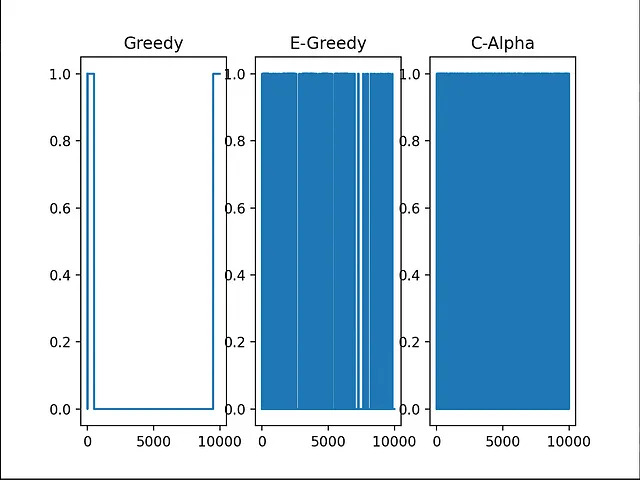
\includegraphics[height=4.5cm]{Pictures/deep-reinforcement-learning/greedy-vs-e-greedy-vs-c-alpha.jpg}
    \caption{Greedy (0.09) VS $\epsilon$-Greedy (0.37) VS Constant Alpha (0.88)}
\end{figure}

\subsection{Upper-Confidence-Bound (UCB) Action Selection \cite{medium-numsmt2-rl-ch2-part-4}}\label{MAB: Upper-Confidence-Bound (UCB) Action Selection}

One better way to select actions could be to choose them with a preference for the actions that we are less confident about.

Choose which arm to exploit based on how satisfying the reward was, but also with a preference for arms that you’ve exploited less. For an arm that you haven’t tried as much you are less confident about the reward, so you may want to experiment with it more to become more confident about its quality on average. This concept is called Upper-Confidence-Bound Action Selection (UCB).

\[
    A_t = \arg\max_a \left[ Q_t(a) + c \sqrt{\displaystyle\dfrac{\ln(t)}{N_t(a)}} \right]
\]

Interpretation:
\begin{enumerate}
    \item $A_t$ is the action at time $t$, selected as the action that maximizes the formula in between the brackets.
    \item $Q_t(a)$ is the estimated value of the action
    \item The right side of the equation in the brackets can be thought of as a representation of the uncertainty of what the reward will be for any given action.
    \item $N_t(a)$ is the number of times this action has been selected. Since it’s in the denominator, as it increases it causes the value on the right side to shrink. This encapsulates the concept that as we select an action more we become less uncertain of its value.
    \item $\ln(t)$ denotes the natural logarithm of $t$ which is the current timestep. As $t$ rises our uncertainty increases but slower over time as per the natural log function.
    \item The parameter $c$ (constant in range $[0, 1]$) can be be considered as determining the \textbf{degree of exploration}. Higher $c$ values cause greater exploration because they cause the uncertainty about actions to be larger.
\end{enumerate}


\section{Gradient Bandit Algorithms \cite{medium-numsmt2-rl-ch2-part-5}}\label{MAB: Gradient Bandit Algorithms}

As opposed to action-value methods that estimate the value of actions, gradient bandit methods don’t care about the value of an action but rather learn a preference for each action over another.

This preference has no interpretation in terms of reward. only the relative preference over other actions matters.

The probability of selecting any action is given according to a \textbf{soft-max distribution} (SEE: \fullref{Softmax function}):
\[
    \pi_t(a) = Pr\dCurlyBrac{A_t = a} = P(A_t=a) = \displaystyle\dfrac{e^{H_t(a)}}{\dsum_{i=1}^{k} e^{H_t(i)}}
\]

\begin{enumerate}
    \item The set of numbers are the actions, so each action will be given a probability of being selected and the probabilities of all those actions will sum to 1.
    \item For example, if there are 3 actions and the game is at some timestep $t$ you could have: $\pi_t(1) = 0.3$, $\pi_t(2) = 0.6$, $\pi_t(3) = 0.1$.
    \item The value $H_t(a)$ represents the preference of selecting an action a over the other actions.
\end{enumerate}

\vspace{0.2cm}

On each step, after selecting the action $A_t$ and receiving the reward $R_t$, the action preferences are updated:
\[
\begin{aligned}
    H_{t+1}(a) &= 
    \begin{dcases}
        H_t(a) + \alpha(R_t - \bar{R_t})(1-\pi_t(a)) & \text{if } a = A_t \\
        H_t(a) - \alpha(R_t - \bar{R_t})\pi_t(a) & \text{for all } a \neq A_t
    \end{dcases}
\end{aligned}
\]

\begin{enumerate}
    \item The top part of the equation represents the preference update for the action just taken and the bottom part represents the preference updates for all other actions.
    \item $\alpha > 0$ is a step-size parameter that determines the degree to which the preferences are changed at each step
    \item $\bar{R_t}$ or “$R$ mean at timestep $t$” is the average of all the rewards from all timesteps including timestep $t$ for $A_t$. Similar to previous methods, this can be updated using incremental updates with the sample-averaging method or a constant-$\alpha$ parameter that is better suited for nonstationary rewards.
    \item $\bar{R_t}$ can be thought of as a baseline against which the current reward is compared. If the reward is higher than the baseline, then the preference for this action is increased. If the reward is lower than the baseline, then vice-versa.
    \item The bottom part of the equation moves the preferences for all other actions in the opposite direction.
\end{enumerate}


\section{Associative Search (Contextual Bandits) \cite{medium-numsmt2-rl-ch2-part-6, kaggle-parsasam-reinforcement-learning-notes-multi-armed-bandits}}\label{Associative Search (Contextual Bandits)}

The variations of the k-armed bandits problem we’ve seen thus far have been nonassociative: we haven’t had to associate different actions with different situations. In \textbf{nonassociative tasks}\indexlabel{MAB: nonassociative tasks}, the agent tries to find a single best action if the reward is stationary, or to track the best action over time if the reward is nonstationary.

\textbf{Associative search task} involves both trial-and-error learning to search for the best actions, and association of these actions with the situations in which they are best. Associative search tasks are often called \textbf{contextual bandits}.









































































